% Drawing 152/01-13 -- folder 152, batch 01, archive page 1 (PDF page 2).
% Transcription: en haut, entre la chaîne $s_0 \dots s_4$ et les cercles de droite, au crayon : un cercle pâle portant cinq marques épaisses, deux secteurs noircis issus de son centre, à gauche et à droite, prolongés de traits épais, et quatre longs traits fins passant par le centre.
% Kind: faint circle with five rim marks, two blackened wedges, lines through the centre. Method 2 (schematic redraw from the facsimile). Status: ok.
% Notes: The faint circle (an ellipse fitted to his), five heavy marks on it (top, left, right, lower right, lower left), the two blackened wedges with their apex at the centre, one to the left and one to the upper right, each continued by heavy strokes beyond the circle (at the left a long stroke along its lower side and a short one at its upper tip, at the right three strokes), and four thin lines ending at or passing through the centre (from the upper left, from the top to the bottom, from the lower left, to the lower right), all drawn through one computed centre. The wedges are scribbled black on the page, their outline not sharp: they are drawn as filled triangles covering the densest part of the scribble. Not drawn: the ink line of the list's frame passing under the figure. Redrawn 2026-11-12 (issue 128). Overlay check 2026-11-14 (claude-opus-5-5, issue 147): the 400 dpi colour rendering of the 402 ppi scan laid under the redraw, rasterised from its TikZ (not compiled: no TeX in the session). The left wedge and its strokes were up to 2.5 units off the scribble (the long lower stroke started at the wedge instead of running along it to the apex): moved onto the ink; the circle, its marks, the right wedge and the four lines lie on their ink within about 1 unit and are kept. Matches the facsimile.
% Coordinates: 1 unit = 1 mm = 1/100 of the crop width (bbox in page fractions: [0.59, 0.095, 0.69, 0.19]).
% Redrawn by Claude (claude-fable-5-2), issue #128, 2026-11-12; not checked by a human; not compiled (no TeX in the session).
% Checked by Claude (claude-opus-5-5) 2026-11-14 (issue #147): overlaid on the colour scan (402 ppi, rendered at 400 dpi) and corrected; not compiled (no TeX in the session), rasterised for the overlay by a Python reader of this TikZ. Status: ok.
% Rights: reproduces part of the work -- behind RENDER_TRANSCRIPTS, never published by itself.
\documentclass[tikz,border=3pt]{standalone}
\usepackage{amsmath,amssymb}
\usetikzlibrary{patterns,arrows.meta}
\tikzset{pencil/.style={black!45}, struck/.style={black!35}, mpt/.style={circle,draw,inner sep=1.3pt}, pt/.style={circle,fill,inner sep=0.9pt}, opt/.style={circle,draw,fill=white,inner sep=1.1pt}}
\begin{document}
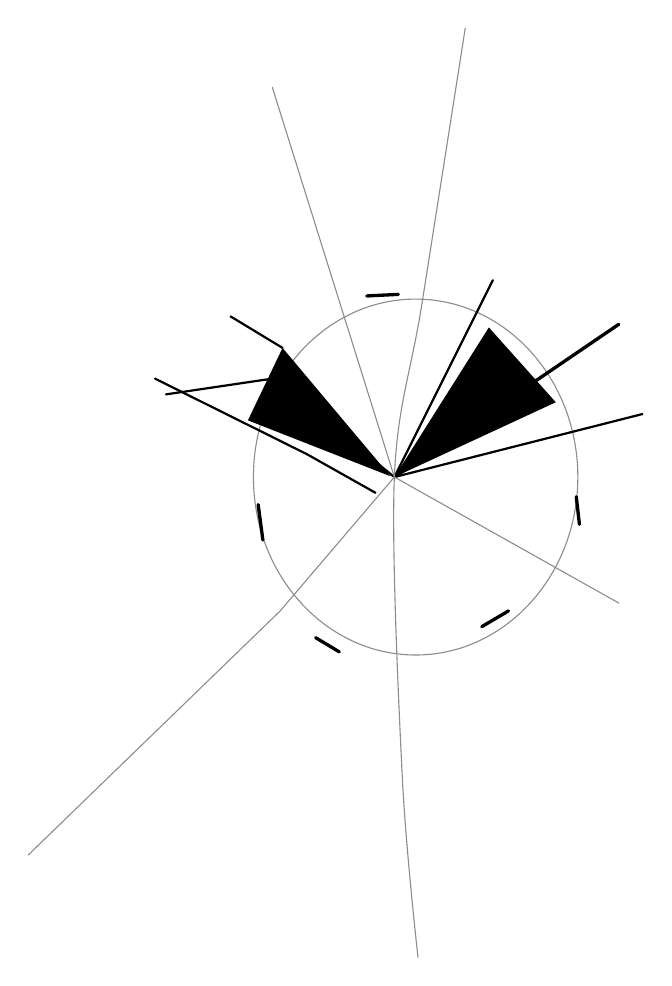
\begin{tikzpicture}[x=1mm,y=1mm,line cap=round,line join=round,font=\small]
\draw[pencil] (54.2,-62) ellipse[x radius=20.6, y radius=22.6];
\draw[very thick] (48,-39) -- (52,-38.8);
\draw[very thick] (34.2,-65.5) -- (34.8,-70);
\draw[very thick] (74.6,-64.5) -- (75,-68);
\draw[very thick] (62.6,-81) -- (66,-79);
\draw[very thick] (41.5,-82.4) -- (44.5,-84.2);
\fill (51,-61.9) -- (37.3,-45.6) -- (32.9,-54.8) -- cycle;
\draw[thick] (21.1,-49.5) -- (40.4,-59.1) -- (49.1,-64);
\draw[thick] (37.3,-45.6) -- (30.7,-41.6);
\draw[thick] (51.5,-62) -- (36,-49.5) -- (22.5,-51.5);
\fill (51.5,-62) -- (63.5,-43) -- (72,-52.5) -- cycle;
\draw[thick] (51.5,-62) -- (64,-37);
\draw[very thick] (51.5,-62) -- (80,-42.6);
\draw[thick] (51.5,-62) -- (83,-54);
\draw[pencil] (36,-12.5) -- (51.5,-62);
\draw[pencil] plot[smooth, tension=0.55] coordinates {(60.5,-5) (55,-40) (51.5,-62) (52.5,-100) (54.5,-123)};
\draw[pencil] (5,-110) -- (37,-79) -- (51.5,-62);
\draw[pencil] (51.5,-62) -- (80,-78);
\end{tikzpicture}
\end{document}
